\documentclass[12pt]{book}
\usepackage[T1]{fontenc}
\usepackage[utf8]{inputenc}
\usepackage[spanish]{babel}
\usepackage{amsmath}
\usepackage{MnSymbol}
\usepackage{wasysym}
\usepackage{multicol}
\setlength{\columnsep}{1cm}
\usepackage[margin=2.5cm,left=3cm, includehead]{geometry}
\usepackage{graphicx}
\usepackage{float}
\usepackage{fancyhdr}
\usepackage{cancel}
\usepackage{pgf,tikz}
\usepackage{mathrsfs}
\usetikzlibrary{arrows}
\usepackage{amsthm}
\usepackage{amsfonts}
\renewcommand{\baselinestretch}{1.5}

% Theorems and definitions
\theoremstyle{plain}
\newtheorem{theorem}{Teorema}[chapter]
\newtheorem{exercise}[theorem]{Ejercicio}
\newtheorem{proposition}[theorem]{Proposición}
\newtheorem{definition}[theorem]{Definición}
\newtheorem{corolary}[theorem]{Corolario}
\newtheorem{obsservation}[theorem]{Observación}
\newtheorem{example}[theorem]{Ejemplo}
\newtheorem{lemma}[theorem]{Lema}

%% NEW Comands
\newcommand{\R}{\mathbb R}  
\newcommand{\N}{\mathbb N}  
\newcommand{\Z}{\mathbb Z}  


\begin{document}
\title{Tesis primera parte.}
\author{Jorge Ballote}
\thispagestyle{plain}
\pagenumbering{Roman}


% \input{agradecimientos.tex}
% \input{resumen.tex}
\newpage
\pagenumbering{arabic}
    \chapter{Planeación}
    Éste no es un capítulo de la tesis. Sólo está en el mismo documento para tener mis ideas apuntadas.
    He decidido que los capítulos del "libro" deben cubrir los siguientes temas. El órden y la distribución de los capítulos están sujetos a cambios.
    \begin{enumerate}
        \item \textbf{Estado del arte:} Aquí irán los estudios que preceden al mío. Incluso pienso escribir resultados previos para clasificación de pollen. 
        \item \textbf{Preeliminares:} Con el objetivo de que este trabajo sea autocontenido, pretendo escribir cualquier tema que se use en algún capítulo. En ésta sección sólo se mencionarán algunos temas, sin necesidad de indagar a fondo en ellos. Ejmplos de esto podrían ser \textsl{Fully Connected Network} o algunos resultados de cálculo variacional o Ecuaciones diferenciales.
        \begin{enumerate}
            \item Series de Taylor
        \end{enumerate}
        \item \textbf{Redes neuronales convolucionales:} Una explicación de cómo funcionan. De cómo están construídas y la notación matemática destras de éstas. Me gustaría hacer énfasis en que una convolución $X*k$ puede ser visto como una multiplicación de matrices $Ax$.
        \item  \textbf{Métodos de ecuaciones diferenciales:} El objetivo en este capítulo es describir los métodos más comunes de ecuaciones diferenciales, cómo lo son Euler, El método del trapecio o Runge Kutta. Quizá incluso se podría tomar en cuenta los estudios de estabilidad de los métodos.
        \item  \textbf{Teoría de control óptimo.} Una breve explicación del control óptimo. El principio del máximo de Pontryagin, las ecuaciones de Hammilton Bellman. Los métodos de resolución comunes, como el shooting method. Y sobre su relación con el entrenamiento de una red neuronal.
        \item \textbf{ResNet:} Tanto la explicación de una, como su interpretación como discretización de una ODE.
        \item \textbf{Estudio de la estabilidad de redes neuronales:} Éste capítulo está dedicado para los resultados teóricos que obtengamos como resultado de crear una arquitectura nueva, o modificar la ResNet.
        \item  \textbf{Experimentación;} Los resultados de nuestra arquitectura comparada con otras arquitecturas en el estado del arte.
        \item \textbf{Conclusiones:} Un breve resumen de los resultados obtenidos.
    \end{enumerate}
    No necesariamente son 9 capítulos. Algunos podrían entrar dentro de los preeliminares y algunos puntos podrían formar un sólo capítulo en conjunto.

    
    %%%%%%%%%%%%%%%%%%%%%%%%% CHAPTER 
    %%%%%%%%%%%%%%%%%%%%%%%%%%%%%%%%

    \chapter{Preeliminares}
    \begin{definition}[Big O notation]
        Sean $f$ y $g$ funciones $f,g:\mathbb N \to \mathbb R^+$. Decimos que $f(n) = \mathcal O(g(n))$ si existen enteros positivos $c$ y $n_0$ tales que para cualquier entero $n\geq n_0$,
        \begin{equation}
            f(n) \leq cg(n).
        \end{equation}
        Cuando $f(n) = \mathcal O(n)$, decimos que $g(n)$ es una cota asintótica superior de $f(n)$,
    \end{definition}
    \textcolor{red}{traducir Big O notation}

    \begin{definition}[Polinomio de Taylor]
        Sea $f$ una función $n$ veces diferenciable, y sean $$a_k = \frac{f^{(k)}(a)}{k!}.$$
        Definimos el Polinomio de Taylor de grado $n$ para $f$ en $a$ como
        $$P_{n,a}(x) = a_0 + a_1(x-a) + \cdots + a_n(x-a)^n.$$
    \end{definition}
    El polinomio $P_{n,a}(x)$ ha sido definido de manera que $P_{n,a}(a) = f^{(k)}(a)$ para $0\leq k \leq n$.
    \begin{definition}
        Sea $f$ una función tal que $P_{n,a}(x)$ existe, definimos el \textcolor{blue}{término de residuo} $R_{n,a}(x)$ como 
        \begin{equation}
            R_{n,a}(x) = f(x) - P_{n,a}(x).
        \end{equation} 
    \end{definition}
    \begin{theorem}[Teorema de Taylor]
        Supóngase que $f^{(1)}$, $f^{(2)}$, ..., $f^{(n+1)}$ están definidos en $[a,x]$. Entonces 
        \begin{equation}
            R_{n,a}(x) = \frac{f^{n+1}(t)}{(n+1)!}(x-a)^{n+1}
        \end{equation}
        para algún $t\in (a,x)$.
    \end{theorem}


    \section{Inteligencia artificial y Aprendizaje profundo.}
    El \textsl{Aprendizaje de Máquina} es un caso particular de la inteligencia artificial, en donde la máquina aprende de los datos proporcionados. Para ello es importante definir qué significa aprender \cite{Mitchell}.
    \begin{definition}
        Se dice que un programa de computadora aprende de la experiencia $E$ respecto a un conjunto de tareas $T$ y medida de rendiminto $P$ si el rendimiento en las tareas en $T$, medido con $P$ mejora gracias a la experiencia $E$.
    \end{definition}
    %%%%%%%%%%%%%%%%%%%%%%%%% CHAPTER %%%%%%%%%%%%%%%%%%%%%%%%%%%%%%%%

    \chapter{Introducción a las redes neuronales convolucionales}
    La literatura de las redes neuronales data desde \textcolor{red}{inserte fecha}. Sin embargo, no fue hasta el \textcolor{red}{2015} con la introducción de las \textsl{redes neuronales convolucionales} (CNN por sus siglas en inglés) \textcolor{blue}{que la comunidad científica empezó a prestar especial atención}. Para entender a profundidad a las CNNs, definiremos lo que es una convolución. Para un estudio más detallado es posible consultar \cite{CNNdefinition,deeplearningbook}. En matemáticas, se suele referir a la convolución de dos funciones $f$ y $g$.
    \begin{definition}[Convolución]
        Sean $f,g : \R \to \R$. La convolución de $f$ con $g$, denotada como $f * g$ se define como:
        $$(f*g)(t) = \int_{0}^t f(\tau)g(t-\tau)d\tau$$
    \end{definition}
    Ésta definición sin embargo no es muy práctica para los paradigmas computacionales, pues  las limitaciones físicas nos obligan a traducir la integral como una \textcolor{red}{suma de intervalos muy pequeños}. Además, si tomamos $f$ como una imagen, es necesario considerar más de una dimensión.
    \begin{definition}[Convolución de una imagen con un kernel]
        Sea $I$ una imagen y $K$ un kernel bidimensional. La convolución de $I$ con $K$ es la imagen $(I*K)$ definida como:
        $$(I*K)(i,j) = \sum_m\sum_n I(m,n)K(i-m,j-n).$$ 
    \end{definition}
    En varias librerías de aprendizaje automático se implementa una correlación cruzada en lugar de una convolución. La única diferencia entre una correlación cruzada y una convolución es la orientación del Kernel. En este trabajo, adoptaremos la convención usual de referirnos a las correlaciones como convoluciones.
    \begin{definition}
        Sea $I$ una imagen y $K$ un kernel bidimensional. La correlación cruzada de $I$ con $K$ es la imagen definida por 
        $$(I*K)(i,j) = \sum_m\sum_n I(i+m,j+n)K(m,n).$$ 
    \end{definition} 

    \begin{figure}[H]
        \centering
        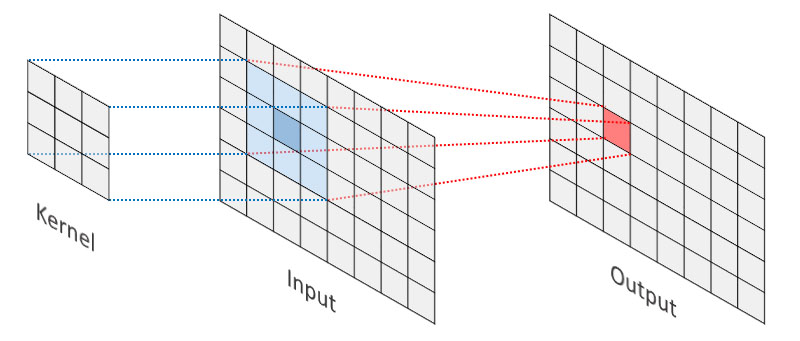
\includegraphics[width=4in]{../src/ch1convolution.jpg}
        \caption{Representación gráfica de una convolución. Para cada posición del Kernel sobre la imagen, se realiza una multiplicación \textsl{entrada por entrada} del Kernel y la un conjunto de pixeles de la imagen, del mismo tamaño que el Kernel.}
    \end{figure}
    % \begin{definition}
    %     Sea $x$ una característica en $\mathbb R^{h\times w}$ y $K$ un filtro de $(2r + 1) \times (2r+1)$. La \textsl{convolución por canal} de $x$ y $K$, a la cual denotaremos $y:= K \bigotimes x$, es una característica en $\R ^{h \times w}$ tal que:
    %     \begin{equation}
    %         y_{i,j} :=  \sum_{l,k=-r}^r K_{l+r+1, k+r+1} x_{i+l, j+k} 
    %     \end{equation}
    %     para todo $i = 1,2,..., h$ y $j = 1,2,..., w$.
    % \end{definition}

    % Es posible extender esta definición para, filtros de $2r\times 2r$, sin embargo, los tamaños más comunes de kernels son $3\times 3$ y $5\times 5$.
    %%%%%%%%%%%%%%%%%%%%%%%%% CHAPTER 1%%%%%%%%%%%%%%%%%%%%%%%%%%%%%%%%

    \chapter{Teoría de control óptimo}
    
    Cuando hablamos de sistemas, nos referimos a un proceso que cambia de estado conforme pasa el tiempo. En nuestro caso pensemos en un sistema dinámico definido en el intervalo $[0, T]$ como
    \begin{equation}
        \label{ch2system}
        \dot x =f(x(t),t), \quad x(0) = x_0,  
    \end{equation}
    donde $x(t)$, conocida como la \textsl{variable de estado} puede representar la producción de alimento en un tiempo $t$, el dinero recaudado en un tiempo $t$, o en general el estado de un proceso en un tiempo $t$. En logística y física, existen variables que podemos controlar, como la cantidad de publicidad, o la reinversión de capital cada cierto momento. Con lo que podemos extender nuestro sistema  (\ref{ch2system}) al siguiente:
    \begin{equation}
        \label{ch2controlsystem}
        \dot x = f(x(t),u(t),t), \quad x(0) = x_0,
    \end{equation}
    donde la variable $u(t)$ es denominada \textsl{variable de control}. Conociendo la variable de control, es posible determinar la solución para $x$ en el sistema (\ref{ch2controlsystem}). El problema de control óptimo reside en maximizar la \textsl{función objetivo}, definida como
    \begin{equation}
        J = \int_0^T F(x(t), u(t), t)dt + S[x(T), T].
    \end{equation}
    Donde $F$ puede es conocida como \textcolor{red}{cómo es conocida} y la función $S$ determina el \textcolor{red}{traducir salvage} en el estado final $x(T)$ en el tiempo $T$. Se denotará al conjunto de calores posibles de $u(t)$ como $\Omega(t)$.

    \begin{definition}
        El \textsl{problema de control óptimo} es encontrar un valor admisible $u^*$ tal que 
        \begin{equation}
            \label{ch2umax}
            u^* = \max_{u(t)\in \Omega(t)}\left\{\int_0^T F(x, u, t)dt + S(x(T), T)\right\}
        \end{equation}
        con la condición 
        \begin{equation}
            \label{ch2dynamicCondition}
            \dot x = f(x,u,t), \quad x(0) = 0.
        \end{equation}
        La trayectoria óptima denotada como $x^*$ es la trayectoria que se obtiene cuando $u = u^*$.
    \end{definition}

    \section{La ecuación de Hamilton-Jacobi-Bellman}
    Sea $V: \R^n \times \R \to \R$ una función definida por
    \begin{equation}
        V(x,t) = \max_{u(s)\in \Omega(s)}\left\{\int_0^T F(x(s), u(s), s)ds + S(x(T), T)\right\}
    \end{equation}
    donde $s \geq t$.
    \begin{definition}
        Considérese el sistema (\ref{ch2umax})-(\ref{ch2dynamicCondition}). Diremos que el hamiltoniano $H: \R^n\times \R^m \times \R^n \times \R \to \R$ del sistema como 
        \begin{equation}
            H(x,u,\lambda, t) = F(x,u,t) + \lambda f(x,u,t).
        \end{equation}
    \end{definition}
    \section{Ecuación adjunta}
    \section{Principio del Máximo}
    %------------- Notas del capítulo
    \section{Notas del capítulo}
    \begin{enumerate}
        \item Añadir el libro de Suresh P. Sethi. Optimal Control Theory a las referencias.
    \end{enumerate}

    \chapter{Notas}
    \begin{enumerate}
        \item La notitas rojas son cosas que aún deben investigarse o cambiarse. Las notas azules representan textos que no están mal, pero que pueden escribirse de una mejor manera.
        \item En preeliminares pretendo definir lo que es una imagen (una función) y un kernel.
    \end{enumerate}

% \input{optimal.tex}
% \appendix
% \input{apendix1.tex}

\bibliographystyle{unsrt}
\bibliography{../main/papers.bib}
    

\end{document}